\documentclass[11pt]{article}

\usepackage[top=0.5in, bottom=0.5in, left=0.5in, right=0.5in]{geometry}
\usepackage{floatrow}
\usepackage{authblk}
\usepackage{filecontents,catchfile}
\usepackage{hyperref}
\usepackage[utf8]{inputenc}
\usepackage{amsmath}
\usepackage{amsfonts}
\usepackage{amssymb}
\usepackage{siunitx}
\usepackage{graphicx}
\usepackage{subcaption}
\usepackage{float}
\usepackage[nottoc,numbib]{tocbibind}
\usepackage{biblatex}

\bibliography{references.bib}

\newfloatcommand{capbtabbox}{table}[][\FBwidth]

\title{Sentiment and Bias Analysis over News Data on Social Media}
\author{Mohammad Mahdi Abdollahpour}

\makeatletter
\let\inserttitle\@title
\let\insertauthor\@author
\makeatother

\begin{document}

\begin{center}
  \LARGE{\inserttitle}
  \vskip 0.8em
  \large{NLP Project Phase 2 Report}
  \vskip 0.8em
  \small{\insertauthor}
\end{center}

\section{Overview}
The goal of this phase is to conduct some experiments with the data collected previously. These experiments include training language models separately on each class and the whole data, training multiple classification models to predict bias on a given headline, and finally to get some insights about the inners of the models using some interpretation techniques.


\section{Word Vector Similarities}
\texttt{spaCy} library provides a tool to calculate the similarity between two documents based on \texttt{word2vec} embeddings.\footnote{https://spacy.io/usage/linguistic-features\#vectors-similarity} I used \texttt{pandas} to sample a fraction of data from each class multiple times and calculate the similarity between each pair of sample documents and finally calculate the average of similarities between every pair of classes to see whether the word choices are any different between different classes. Cosine similarities have been exponentiated to make the differences more noticeable.

\begin{center}
  \begin{tabular}{ccc}
    \hline
    \textbf{Class 1} & \textbf{Class 2} & \textbf{Cosine Similarity Average}\\
    \hline
    \hline
    -2 & -1 & 2.7099 \\
    -2 &  0 & 2.7054 \\
    -2 &  1 & 2.7089 \\
    -2 &  2 & 2.7147 \\
    -1 &  0 & 2.7154 \\
    -1 &  1 & 2.7163 \\
    -1 &  2 & 2.7082 \\
     0 &  1 & 2.7150 \\
     0 &  2 & 2.7049 \\
     1 &  2 & 2.7096 \\
    \hline
  \end{tabular}
  \end{center}

Implementation is available under \texttt{notebooks/exploratory} directory.

\section{Dependency Parsing \& NER}
I used \texttt{spaCy} to get dependency parsing and named entity from some sample sentences. Some output examples of this tool on my data are provided in the next page. To investigate the implementation and see more examples check out the notebook under \texttt{notebooks/exploratory} directory.

\newpage

\begin{center}
  \begin{figure}[h!]
    
\includegraphics[width=0.85\textwidth]{figs/dep_ner/dep_2.png}
  \end{figure}
\end{center}

\begin{center}
  \begin{figure}[h!]
    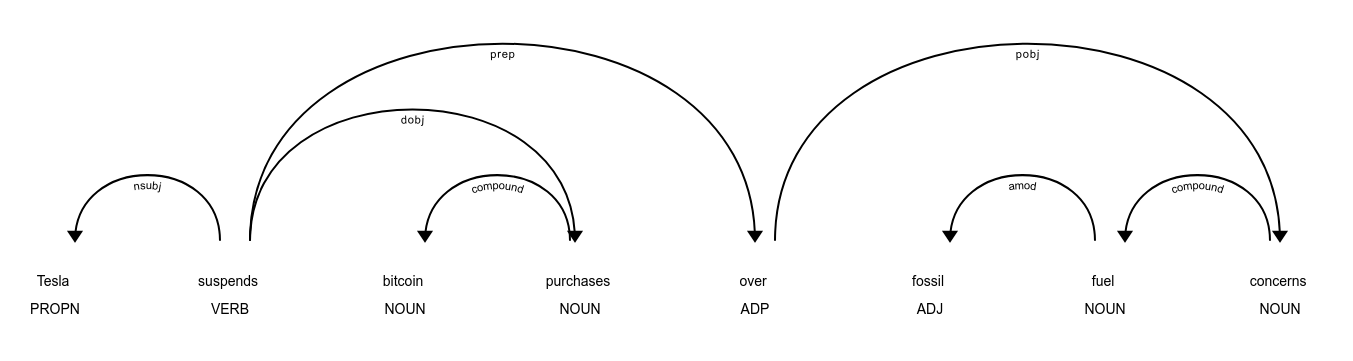
\includegraphics[width=0.85\textwidth]{figs/dep_ner/dep_1.png}
  \end{figure}
  \end{center}

\begin{center}
  \begin{figure}[h!]
    
\includegraphics[width=0.35\textwidth]{figs/dep_ner/ner_1.png}
  \end{figure}
\end{center}

\begin{center}
  \begin{figure}[h!]
    
\includegraphics[width=0.55\textwidth]{figs/dep_ner/ner_3.png}
  \end{figure}
\end{center}

\begin{center}
  \begin{figure}[h!]
    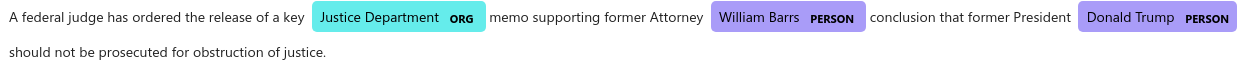
\includegraphics[width=0.95\textwidth]{figs/dep_ner/ner_2.png}
  \end{figure}
\end{center}

\newpage

\section{Language Model}
Several types of language models have been introduced in the field of Natural Language Processing. Two widely used LMs are Causal Language Model (CLM) and Masked Language Model (MLM). In this phase, I have fine-tuned one model for each of these two types.

\subsection{Fine-Tuning LMs}

\paragraph{GPT2 as a CLM}
According to the architecture, GPT2 has a uni-directional nature which is sometimes called causal as it does not know anything about future words in the sequence at the time of predicting the next word. This type of inference architecture is most similar to the classic statistical models and is well-known among NLP practitioners.
\newline
I modified and used the script provided in the HuggingFace github repository to fine-tune GPT2 CLM on my data. More precisely, I trained this model on each class to see whether it can capture the differences and biases present in the dataset. In the following table the perplexity of the model after training 3 epochs is provided.

\begin{center}
\begin{tabular}{cc}
  \hline
  \textbf{Class} & \textbf{Perplexity} \\
  \hline
  \hline
  -2 & 56.39 \\
  \hline
  -1 & 57.53 \\
  \hline
  0 & 53.42 \\
  \hline
  1 & 62.63 \\
  \hline
  2 & 67.50 \\
  \hline
\end{tabular}
\end{center}

More detailed information about fine-tuning the model is available in the \texttt{models} directory.

\paragraph{RoBERTa as a MLM}
RoBERTa which is based on the BERT architecture, is bi-directional in nature. By default, it can not be used to generate sentences in an auto-regressive fashion. However, one can predict masked words in a sentence using this type of LM.
\newline
Same as GPT2, I modified and used the script provided in the HuggingFace github repository to fine-tune RoBERTa MLM on each class. Below is a table providing the perplexity of this model after fine-tuning on each class.

\begin{center}
  \begin{tabular}{cc}
    \hline
    \textbf{Class} & \textbf{Perplexity} \\
    \hline
    \hline
    -2 & 6.12 \\
    \hline
    -1 & 6.04 \\
    \hline
    0 & 6.07 \\
    \hline
    1 & 6.84 \\
    \hline
    2 & 7.74 \\
    \hline
  \end{tabular}
  \end{center}

\subsection{Observations}
\paragraph{Perplexity Trend}
The first finding is that the perplexity has a surprising increasing slope as it goes from class -2 to class 2. We can view this phenomenon in two ways. First, it may have stemmed from a possibility that lesser amount of news from conservative media was present in the data fed into these two models at the time of pre-training. Second, it may indicate that left-handed media are more consistent in crafting and publishing news. Also, one can argue that aside from consistency, their claims are more in-line with the texts published on other sources like wikipedia.

\paragraph{Samples from Generated Texts}
I fed some incomplete phrases to the models to find if it can mimic the style and biases of each side of the political spectrum and found some interesting results.
\newline
For example, we know that conservative media has always backed the Second Amendment to the United States Constitution which basically is a permission for people to buy guns. On the other hand left-handed media have been against it and always tried to draw a negative picture of this law.
Interestingly, RoBERTa has captured this bias as we can see in the following result:

\begin{center}
  \begin{tabular}{cccc}
    \hline
    \textbf{Fine-Tuned on Class} & \textbf{Input Phrase} & \textbf{Model Output} & \textbf{SoftMax Score} \\
    \hline
    \hline
    2 & Guns should be [mask] & Guns should be legal & 0.30 \\
    1 & Gun laws [mask] people & Gun laws protect people & 0.214827 \\
    -2 & Guns should be [mask] & Guns should be banned & 0.31 \\
    -2 & Gun laws [mask] people & Gun laws hurt people & 0.325159 \\
    \hline
  \end{tabular}
\end{center}

All of the generated texts during experiments are available in the directory \texttt{docs/phase\_2\_report/figs}.

\section{Classification}
I defined and trained several models to classify news headlines based on their source bias. For training all of those models I used \texttt{MSE} as the loss function. It means that I viewed the problem as a regression problem. In other words, the model should output a number between -2 and 2 which means that there is basically two classes instead of 5 classes. This is mainly because based on the definition of the classes (biases), they have a natural order. There is a spectrum of biases, hence the problem is really a regression one not a typical classification like cats vs. dogs.

\paragraph{word2vec + BiLSTM}
The best \texttt{word2vec} pre-trained model for my use-case was \texttt{word2vec-google-news-300} which I downloaded using \texttt{gensim} api. I provided the \textbf{option for both fine-tuning and freezing the word2vec embeddings} in the code.
On top of \texttt{word2vec} embeddings I used two layers of \texttt{BiLSTM} with hidden size of 256 and on top of that two layers of \texttt{BiLSTM} with hidden size of 128. Then I fed the last hidden states of the final layer to a fully connected layer containing 256 neurons. The single scalar output of this network is then fed to a \texttt{tanh} activation multiplied by 2 which enforces the final output to be between -2 and 2.
Both \texttt{BiLSTM} layers use 20 percent of dropout. I also used gradient clipping in the training loop to avoid gradient explosion.
To calculate the accuracy I mapped the output in range $(-\infty, -1.5)$ to -2 and the output in range $[-1.5, -0.5)$ to -1 and so on.

\paragraph{BERT + BiLSTM}
There are two main approaches to use \texttt{BERT} for classification. One to use the vector of [CLS] token and the other is to use vectors of each token of sentence other that [CLS]. I used the second approach with two layers of \texttt{BiLSTM} with hidden size of 256 and dropout of 20 percent. And on top, I used a fully connected layer and a \texttt{tanh} to get a number between -2 to 2. I experimented with different number of layers of \texttt{BiLSTM} and fc layers but the best overall result was achieved by the settings I mentioned. I also provided the \textbf{option to both fine-tune or freeze the BERT embedding layer}.

\paragraph{BERT + CNN}
Same as the previous model, I used BERT vectors of each token with zero padding and fed them into a convolutional layer. This layer is a concatenation of four 1D conv layers of sizes 2, 3, 4 and 5 with max-pooling. Then the output is fed into a fully connected layer with tanh activation.

\begin{center}
  \begin{tabular}{ccccccc}
    \hline
    \textbf{Model} & \textbf{Train Acc} & \textbf{Val Acc} & \textbf{Test Acc} & \textbf{Train Loss} & \textbf{Val Loss} & \textbf{Test Loss} \\
    \hline
    \hline
    [Baseline] & 20 & 20 & 20 & - & - & - \\
    w2v + BiLSTM & 90.82 & 31.52 & 26.67 & 0.11 & 2.84 & 3.05\\
    BERT + BiLSTM & 84.7 & 33.6 & 26.95 & 0.14 & 2.16 & 2.6 \\
    BERT + CNN & 75.27 & 27.68 & 21.34 & 0.22 & 2.23 & 2.32 \\
    \hline
  \end{tabular}
\end{center}

The above table shows the results at the checkpoint of best validation accuracy during training. As mentioned in the last report, the dataset is very noisy and it was predicted that the results may be not very desirable. However, \textbf{the outcome should be considered as a draft because the models were trained only on a fraction of data (less that $ \frac{1}{200} $) without any fine-tuning of embedding layers due to time and computational limitations}. More details are available under \texttt{models} directory.

% \section{Interpretation}
% \paragraph{Attention Vectors}

% \paragraph{SHAP}

\end{document}